\documentclass[conference]{IEEEtran}
% \IEEEoverridecommandlockouts
% The preceding line is only needed to identify funding in the first footnote. If that is unneeded, please comment it out.
\usepackage{cite}
\usepackage{amsmath,amssymb,amsfonts}
\usepackage{algorithmic}
\usepackage{graphicx}
\usepackage{textcomp}
\usepackage{xcolor}
\def\BibTeX{{\rm B\kern-.05em{\sc i\kern-.025em b}\kern-.08em
    T\kern-.1667em\lower.7ex\hbox{E}\kern-.125emX}}
\begin{document}

\title{A Distributed Data Layer for Interoperable Scientific Workflows and Web Apps
% *\\
% {\footnotesize \textsuperscript{*}Note: Sub-titles are not captured in Xplore and
% should not be used}
% \thanks{Identify applicable funding agency here. If none, delete this.}
}

% \author{\IEEEauthorblockN{1\textsuperscript{st} Shady El Damaty}
% \IEEEauthorblockA{\textit{dept. name of organization (of Aff.)} \\
% \textit{name of organization (of Aff.)}\\
% City, Country \\
% email address or ORCID}
% \and
% \IEEEauthorblockN{2\textsuperscript{nd} Jakub Smékal}
% \IEEEauthorblockA{\textit{dept. name of organization (of Aff.)} \\
% \textit{name of organization (of Aff.)}\\
% City, Country \\
% email address or ORCID}
% \and
% \IEEEauthorblockN{3\textsuperscript{rd} Kinshuk Kashyap}
% \IEEEauthorblockA{\textit{dept. name of organization (of Aff.)} \\
% \textit{name of organization (of Aff.)}\\
% City, Country \\
% email address or ORCID}
% \and
% \IEEEauthorblockN{4\textsuperscript{th} Caleb Tuttle}
% \IEEEauthorblockA{\textit{OpSci} \\
% United States\\
% caleb@opsci.io}
% }

\author{\IEEEauthorblockN{1\textsuperscript{st} Shady El Damaty}
    \IEEEauthorblockA{\textit{OpSci} \\
    Washington, D.C., USA \\
    0000-0002-2318-4477}\\
    \IEEEauthorblockN{3\textsuperscript{rd} Kinshuk Kashyap}
    \IEEEauthorblockA{\textit{OpSci} \\
    Mangalore, India \\
    0000-0001-7899-7179}\\
    \and
    \IEEEauthorblockN{2\textsuperscript{nd} Jakub Smékal}
    \IEEEauthorblockA{\textit{OpSci} \\
    Durham, UK \\
    0000-0003-4989-4968}\\
    \IEEEauthorblockN{4\textsuperscript{th} Caleb Tuttle}
    \IEEEauthorblockA{\textit{OpSci} \\
    Augusta, USA\\
    0000-0002-8469-2221}
}

\maketitle

\begin{abstract}
 International guidance for scientific data sharing has promoted the establishment of massive data repositories to foster increased collaboration, secondary uses of valuable data, and enhanced rigor. Current data sharing practices rely on centralized architecture for content distribution and access control, limiting their ability to satisfy institutional mandates. Cutting-edge primitives for decentralized autonomous workflows provide design patterns for data commons that allow for coordination across distributed communities. Here we describe a data layer design pattern that wraps web primitives for peer-to-peer data sharing, persistent storage, and programmable access control to link decentralized research communities through web applications running on a shared data substrate. We discuss potential applications, use-cases, and future directions.
\end{abstract}

\begin{IEEEkeywords}
decentralized science, desci, data commons, data workflows, open data, FAIR, open science, distributed networks
\end{IEEEkeywords}

\section{Introduction}
% CT note: Structure of this section: 
        % I. Intro paragraph
        % II. Problems with the State of Scientific Data
        %     i. Fragmented and access controlled data
        %     ii. Data decay
        %     iii. Misaligned structural incentives (do these belong in this paper?)
        %     iv. Lots of data--and more data incoming--we need storage!
        %     v. No universal indexer--lack of Findability
        % III. Towards an Open Science Data Commons
        %     i. intro sentence (maybe delete?)
        %     ii. Open Science practices--initial successes
        %     iii. Call to action: "Scientific data must be discoverable, etc..."
\subsection{State of Scientific Data}
The corpus of scientific data today is fragmented across disjoint siloes within complex regulatory regimes and absent unified mechanisms for access control, sharing, and community governance. An avalanche of scientific data is being produced by distributed networks of researchers, consortia, and public works projects. In aggregation, these data provide a messy but unprecedented and invaluable description of our universe, the planet, and human society. Today, big data is “widely viewed as ushering in a new way of performing research and challenging existing understandings of what counts as scientific knowledge” \cite{sep-science-big-data}. However, several challenges come with discovering, maintaining, and aggregating datasets. 

The frictions presented by fragmented and niche access-controlled data repositories make the tasks of finding and accessing scientific data unnecessarily cumbersome. In a survey of approximately 1,700 researchers, respondents listed the following as top difficulties in discovering and re-using data: data are not available, data are stored in diverse locations, and data search tools are inadequate \cite{Gregory2020Lost}.
% In a survey of approximately 1,700 researchers, 68\% of respondents reported that the biggest hindrance to discovering valuable data is that the “data are not available for download or analysis,” 49\% said the data’s being stored in diverse locations is the primary culprit, and a third cited “inadequate search tools” as the driving difficulty \cite{Gregory2020Lost}. 
Because of these difficulties, researchers must often rely on serendipity or social connections to acquire useful data \cite{Gregory2020Lost}. Many scientific data sources are inaccessible to search engines and stored in poorly documented schemas, making their re-use incredibly unlikely, despite national funding institutions declaring the importance of secondary use. 

Data are routinely lost or become practically unusable due to lack of maintenance \cite{JahnkeAsher}. 
Insufficient technological infrastructure has caused the loss of over 80\% of raw scientific data collected during the 1990s, according to estimates \cite{WienerBronner}. 
The chances of dataset remaining extant falls by 17\% every year, beginning three years after a paper is published \cite{Vines2014}. 
% A lack of standards also results in poor interoperability of datasets, preventing useful comparisons or aggregations across studies.
Even when preserved, data often cannot be used for comparisons or aggregations of studies because the data are stored in different structures.
% CT note: I want to delete the following two sentences. The comment on the replication crisis and the "reason for such data decay" might belong somewhere else. This paragraph is for _the fact that_ data is lost due to lack of maintenance.
The replication crisis is partly due to the fact that many studies’ raw data is not stored and published together with the studies as one unit \cite{Miyakawa2020}. One reason for such data decay is that researchers are not trained and often do not have time to manage their data \cite{TeperekDunning}. 

% CT note: Are structural incentives relevant to this paper, to a technical description of a data commons? These sociological points are important for a comprehensive account of the state of scientific data, but maybe we don't need them here.
% SED: Agreed
% The structural incentives within academic research do not encourage maintenance or sharing of data. Scientists are incentivized to publish papers in high impact journals because impact metrics influence funding and career prospects. Producing high-impact papers, however, requires time, as does maintaining archived datasets. Scientists therefore face a dilemma: Time spent maintaining datasets is time not spent writing new publications. For an individual researcher, there is obvious upside to writing publications but no obvious upside to preserving and sharing data. The misalignment of incentives indirectly contributes to data decay.

% % CT note: I replaced the following paragraph with the above paragraph.
% The structural incentives in place for academic research do not encourage data sharing. Researchers typically do not invest time in archiving or preparing datasets for sharing because “investing time in a project beyond its usefulness for publication is counterproductive, given the high expectations for producing research publications” \cite{JahnkeAsher}. The mismatched incentives are exacerbated by the large up-front costs for creating new datasets. From data collection and curation, to regulatory compliance and anonymization - all require time and effort. Scientists face a critical dilemma: Time spent creating new datasets is time not spent writing new publications. This hurts the metrics used to measure one’s impact in the scientific community. The research ecology around data production, management, and sharing has very misaligned incentives today - a perfect example of Goodhart’s law at play: Scientists are often caught chasing the measure, publications and grant funding, as if it were the target, instead of prioritizing actions that expand the frontier of human knowledge. 

Currently, there are several federally and internationally funded repositories that house thousands of terrabytes of open access data. This number is expected to increase with the recent data sharing mandate issued by the US National Institutes of Health (NIH). Over 300,000 researchers and 2,500 institutions receving NIH funds must include a data-management plan as part of their grant application and commit to make taxpayer-funded data publicly available at the conclusion of their study \cite{Kozlov2022}. However, in practice, access to datasets is typically gated by institutional requirements, affiliations, and legal considerations. Furthermore, much of this data is stored on servers operated by centralized infrastructure providers, such as Amazon. Centralized storage services have been criticized for their lack of security, high costs, intransparent business models, and misaligned long term vision. 

\subsection{A Distribued Science Data Index} Across scientific disciplines, there does not yet exist a unified index that allows datasets, their metadata, and derivative works to be searched, aggregated, and retrieved by open access-reliant scientists. The datalad project has tackled the need for providing a universal indexing mechanism, where individual data providers can host the data on their personal machines and broadcast the entire version history of a dataset to the rest of a distributed network \cite{DataLad}. Datalad utilizes cryptographic hashing and version histories provided by git-annex for binary version control of large and complex datasets. The ability to execute code associated with a dataset to generate derived data using new inputs also allows a degree of functional reproducibility difficult to achieve in practice without the support of containerized environments and binary version control \cite{wagner_hanke_2019}. The power of datalad has been demonstrated through the deployment of complex analytic workflows that aggregate hundreds of terrabytes of scientific data to achieve distinction of hypotheses with significantly small effect sizes \cite{Wagner2021.10.12.464122}.  Despite the ability to power autonomous workflows, datalad was not built to guarantee the availability of a dataset. The software relies on users to host the data on their lab or personal infrastructure. However, users have reported datasets indexed by datalad as having gone missing over time due to the costs associated with upkeep of large datasets.

\subsection{Growing Momentum for Distributed Data Commons}
Efforts toward addressing the issues of access controlled, fragmented, and rotting data have already seen some success, suggesting the importance of a data commons and of adopting best practices for data management.

Open science practices that have emerged to combat the replication crisis have clearly demonstrated the domino effect of data sharing on productivity, scientific rigor, and collaboration. Dataset publishing alongside articles allows researchers to reproduce workflows and aggregate across studies to generate more powerful statistical portraits. Data sharing can reduce the total cost placed on the scientific community by reducing duplication of work and allows researchers, who do not have access to expensive equipment, to conduct research. For example, collecting MRI data is costly, time-consuming, and quality can vary substantially across data collection sites. So, a group that publishes a large MRI dataset collected with standard acquisition protocols can accelerate the field of neuroscience: The new data can be used in metanalyses, and researchers with fewer resources can perform their own analyses on individual subject data \cite{Nature2018}. These benefits were core motivations behind the establishment of common repositories such as OpenNeuro \cite{gorgolewski2017openneuro} and metanalytic platforms such as BrainMap \cite{laird2005brainmap}.

% CT note: I tried to condense the following two paragraphs into the above paragraph. I might have reduced the fidelity of examples, particularly in neuroimaging.
% SE: totally fine

% Open science practices that have emerged to combat the replication crisis have clearly demonstrated the domino effect of data sharing on productivity, scientific rigor, and collaboration. Dataset publishing alongside articles allows researchers to reproduce workflows, and aggregate across studies to generate more powerful statistical portraits than would otherwise be feasible for a single researcher or group. For example, for neuroscientists, collecting MRI data is costly, time-consuming, and quality can vary substantially across data collection sites. So, there are numerous benefits to the entire field when a group publishes a large MRI dataset collected with standard acquisition protocols \cite{Nature2018}. Furthermore, MRI studies are incredibly expensive and can benefit immensely from metanalyses of existing datasets. This need has led to the emergence of metanalytic platforms \cite{laird2005brainmap}. However, these maps only provide smoothed averages of averages and do not allow accurate estimation of statistical effect sizes. Access to individual subject data has been noted as a key concern for neuroimaging and is what has motivated the establishment of common repositories such as OpenNeuro \cite{gorgolewski2017openneuro}. 

% Fields such as genomics and astronomy have established data-sharing practices and repositories that allow researchers in these fields to conduct valuable research even when they might not have access to expensive equipment. Not only is it beneficial to make new data available, but even making old data available can lead to new discoveries (see, for example, \cite{BonasGuarch2018}). Data sharing can also reduce unnecessary duplication of work. It allows reviews of data to be performed in a more timely fashion, something that is crucial during times when public policy relies on urgent findings from the scientific community. The benefits of open data extend even to the careers of the researchers who share their data. Some benefits are “increases in citations, media attention, potential collaborators, job opportunities and funding opportunities” \cite{McKiernan2016}. The benefits of data sharing hint at the direction we should take with how we deal with scientific data. Namely, data archival, open data, and easy access can improve not only scientific output but also the condition of humanity at large.

Today, the state of scientific data is closely coupled to the ability for human society to continue innovating and address existential challenges. The importance of a permanent and interactive record of accumulated knowledge for continued scientific innovation has led to a convergent need for standard data management, archival, and sharing practices. Scientific data must be discoverable, accessible, and interoperable in order to support the growing complexity of modern research. Otherwise, science may suffer a tragedy of overabundance, where data is assumed to be common but actionable knowledge is scarce.

\section{Requirements for a Science Data Commons}
In light of the current state of scientific data, institutional guidance and recommendations have emerged to make digital knowledge repositories and services Findable, Accessible, Interoperable, and Reusable (FAIR; \cite{Wilkinson2016}). FAIR principles immediately lend themselves to distributed, decentralized, digital communities of researchers. A common language and culture for interoperable and accessible digital knowledge artifacts empowers the propagation of information across knowledge silos and increases the rate of innovation. Research organizations utilizing datasets shared with FAIR principles have been demonstrated to converge more quickly to concrete research directions, produce more scientific output, and foster closer collaboration across international boundaries \cite{wise2019implementation, boeckhout2018fair}. 

The application of FAIR as requirements for a research data commons is a natural step in the direction for a machine-readable, semantic web of science - in which the corpus of human knowledge is indexable and available for automation workflows to supplement metanalyses, provide real time monitoring of scientific processes, and that indicate future directions for new experiments \cite{Wilkinson2016}. Data commons and repositories should satisfy several requirements in order to meet the needs of distributed science communities.

The following are the FAIR principles, taken from \cite{Wilkinson2016} and can be taken as design requirements for data commons architecture.

% TODO: Is there a better way to format these?
% Can be a table with an accompanying discussion
\subsection{The FAIR Guiding Principles}
\begin{enumerate}
   \item \textbf{To be Findable:} 
   \begin{itemize}
     \item F1. data are assigned a globally unique and persistent identifier
     \item F2. data are described with rich metadata (defined by R1 below)
     \item F3. metadata clearly and explicitly include the identifier of the data it describes
     \item F4. data are registered or indexed in a searchable resource
   \end{itemize}
   
   \item \textbf{To be Accessible:}
   \begin{itemize}
     \item A1. data are retrievable by their identifier using a standardized communications protocol
     \item A1.1 the protocol is open, free, and universally implementable
     \item A1.2 the protocol allows for an authentication and authorization procedure, where necessary
     \item A2. metadata are accessible, even when the data are no longer available
   \end{itemize}
   
   \item \textbf{To be Interoperable:}
   \begin{itemize}
     \item I1. data use a formal, accessible, shared, and broadly applicable language for knowledge representation
     \item I2. data use vocabularies that follow FAIR principles
     \item I3. data include qualified references to other data
     \item A2. metadata are accessible, even when the data are no longer available
   \end{itemize}
   
   \item \textbf{To be Reusable:}
   \begin{itemize}
     \item R1. meta are richly described with a plurality of accurate and relevant attributes
     \item R1.1. data are released with a clear and accessible data usage license
     \item R1.2. data are associated with detailed provenance
     \item R1.3. data meet domain-relevant community standards
   \end{itemize}
   
\end{enumerate}

Several organizations have provided additional clarifications and practical use-case guidance that place the execution of FAIR principles in the context of transparent governance, accountability, and intellectual ownership. The International Neuroinformatics Coordinating Facility (INCF) has paved the way for community governance and establishment of formal procedures to evaluate standards and best practices that promote FAIR principles in science. Frameworks, such as the Basic Framework on FAIRness of Services \cite{BasicFrameworkv1} \cite{BasicFrameworkv3}, contain recommendations specifically for data service providers. The following are the high-level objectives of the recommendations from \cite{BasicFrameworkv3}.

% TODO: Is there a better way to format these?
\subsection{Basic Framework on FAIRness of Services}
\begin{enumerate}
   \item \textbf{Technically-oriented aspects} 
   \begin{itemize}
     \item \emph{FAIR enablement.} The service enables FAIR data by elevating the FAIRness of digital objects and/or supporting the FAIRification process. FAIR enablement is actively driven through the implementation of community-supported standards and interoperability frameworks.
     \item \emph{Quality of service.} The service is delivered in a reliable, secure, high-quality way, consistent with its specifications.
     \item \emph{Open \& Connected.} The service is operated in a low-barrier and inclusive way; seeking integrations and connections with other services; and championing principles of openness consistent with Open Science and Open Research.
   \end{itemize}
   
   \item \textbf{Socially-oriented aspects} 
   \begin{itemize}
     \item \emph{User-centricity.} The service is managed such that it serves the (possibly evolving) goals of the user community, and maximises usability while minimizing burden.
     \item \emph{Transparency.} The service provider communicates with its user community in a transparent manner.
     \item \emph{Longevity.} The service provider designs the service with a timeframe for the maintenance and sustainability of the service in mind and implements measures accordingly, considering the researchers’ necessity for reproducible research.
     \item \emph{Ethical \& Legal.} The service complies with all applicable legal and ethical guidelines, in a transparent and auditable way.
   \end{itemize}
   
\end{enumerate}

\begin{figure*}[htbp]
\centering
  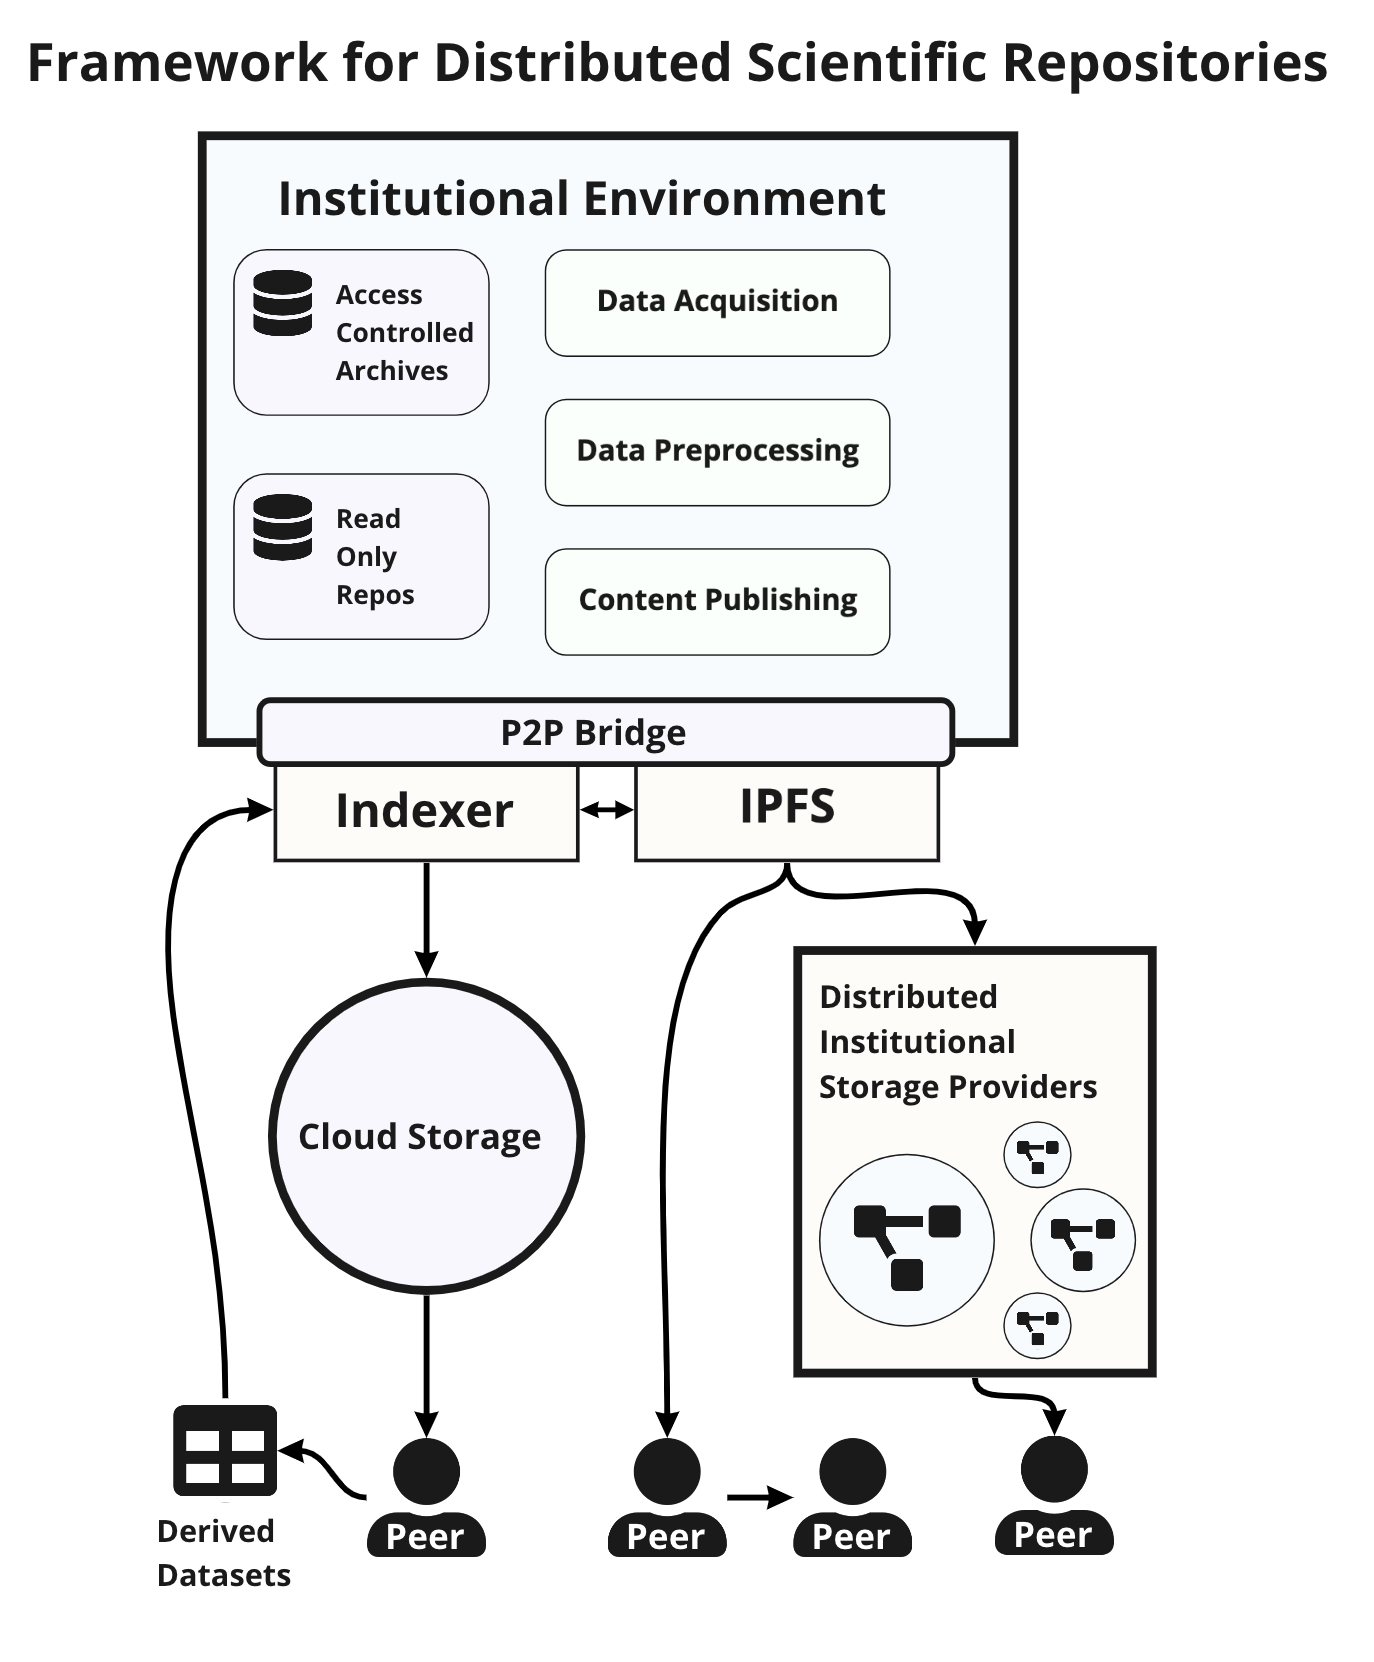
\includegraphics[scale=0.5]{framework.png}
  \caption{Framework for Distributed Scientific Repositories and Content Delivery.}
\end{figure*}

\section{Scientific Workflows \& Mechanisms for Distributed Content Delivery}
The above principles and objectives articulate the broad requirements of a scientific data commons but do not address details of implementation. The acquisition of scientific data typically occurs under the purview of institutions that can provide required infrastructure, expertise, security, and regulatory compliance. Raw data is collected and stored in access controlled archives, typically to protect sensitive information. Data collection pipelines built with FAIR principles in mind will version collected data and provide annotations in the form of standardized metadata descriptions \cite{keator2019tools}. These descriptions are critical for establishing the context in which the data was collected, such as the parameters, experimental protocol, and output dataset structure. An example of FAIR principles in action is the application of the Brain Imaging Data Structure (BIDS) to raw MR images as they come off the scanner and stored as individual frames \cite{gorgolewski2016brain}. Metadata accompanying raw data in access controlled archives, allows individuals to generate secondary derivatives of the original dataset that contain less sensitive information but also retain the necessary context for other collaborators to reproduce their findings. Even so, the complexity of converting raw data into an analyzable format is often taken up by the original custodians of the data. Data preprocessing, in some fields, may be considered an art that requires finessing and specialized hardware to achieve quality results. Individual labs or institutions may seek to provide access to meticulously preprocessed and analyzed datasets utilizing read-only repositories that are hosted on institutional infrastructure and provided to the public, or those with relevant credentials. However, institutions, or individual labs within larger organizations, cannot guarantee indefinite maintenance for self-hosted datasets. 

\begin{figure*}[htbp]
  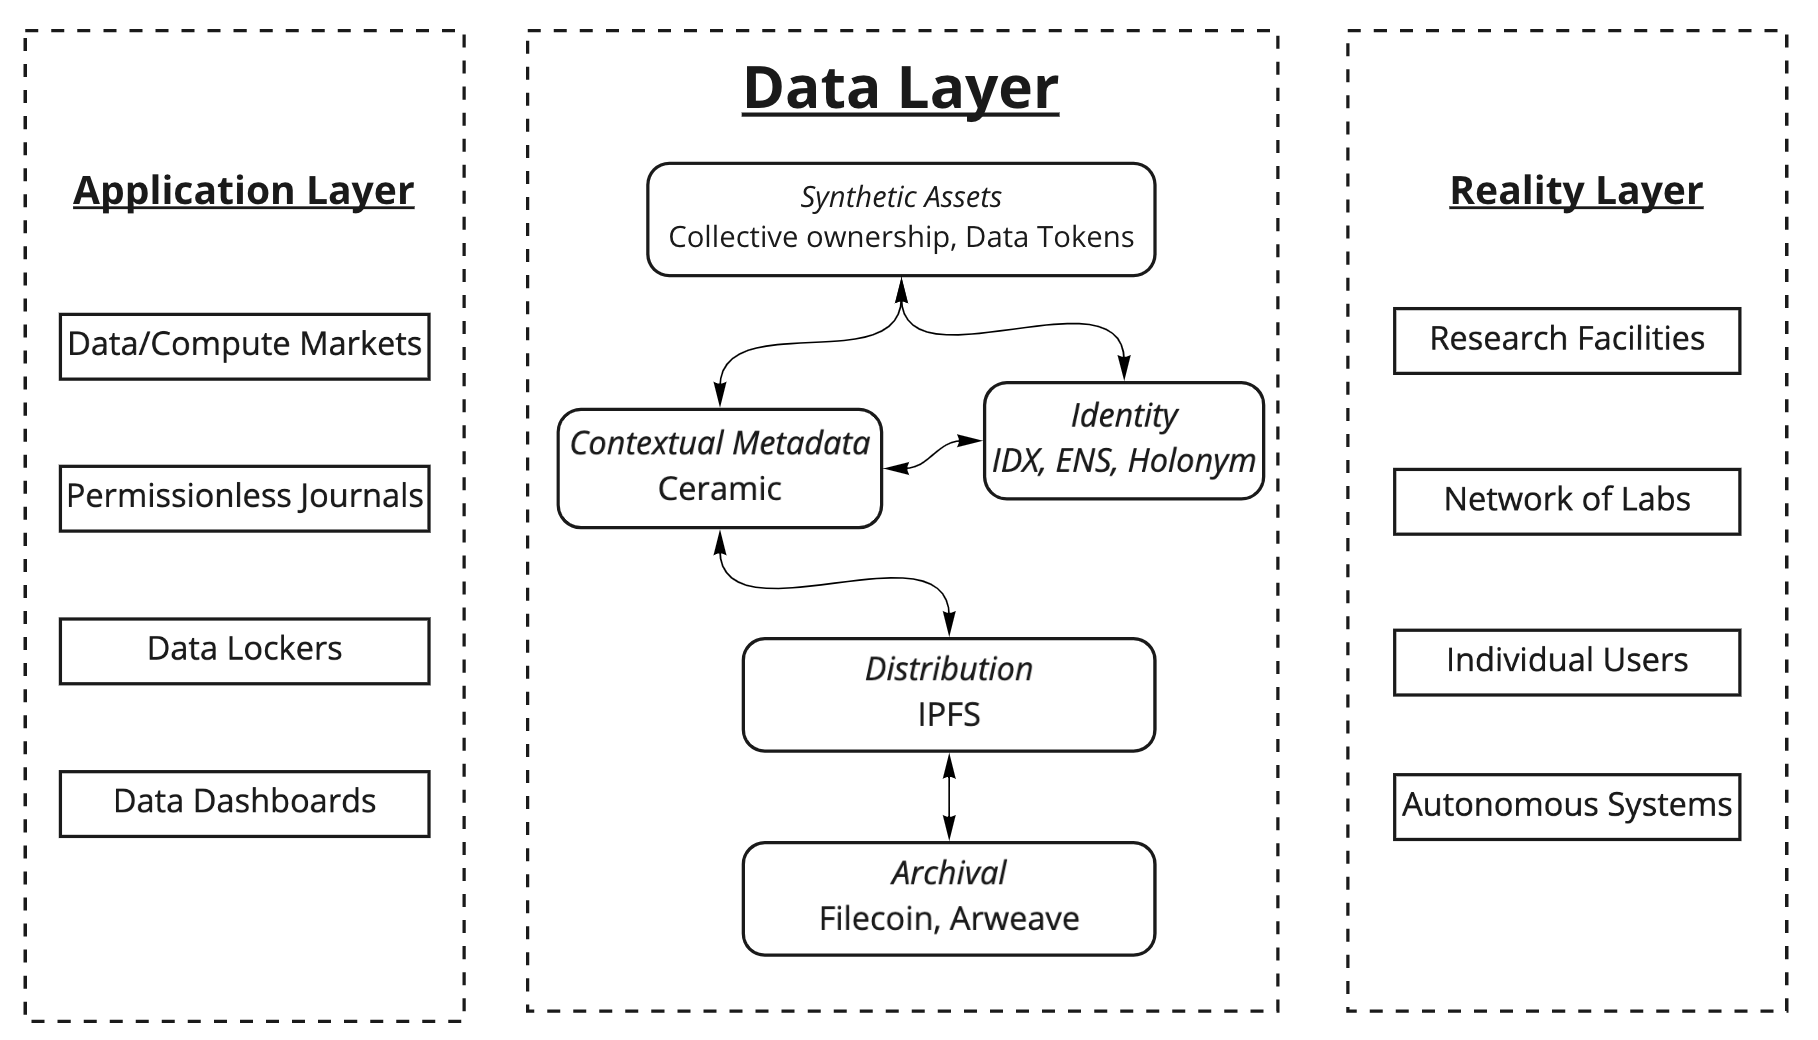
\includegraphics[width=\textwidth]{data-layer.png}
  \caption{Data Layer for Science.}
\end{figure*}

Peer-to-peer protocols can help institutions and laboratories satisfy their requirements for FAIR data sharing during on-going data collection collaborations or at the conclusion of a study. An example schematic appears in Figure 1. A peer-to-peer bridge running within institutional compute infrastructure may be used to establish a connection between other institutions and peers on the internet. The bridge can provide access for public requests, or may be configured to operate only within a closed federation of providers.  A bridge may be composed of an indexer that tracks versions of each dataset, access privileges, associated content, and redundant copies of datasets, or parts of datasets, that are stored by other peers in the network. An individual lab can provide a copy of an index that other peers may access through a centralized storage provider. Peers may use this access to generate derived datasets that can be re-indexed and broadcast to others in the network. However, an index on its own does not satisfy all the requirements for a data commons. An indexer without a data routing protocol must rely on centralized storage providers to broadcast, retrieve, and update their records. A key component for any peer-to-peer bridge is a content-addressable, data routing network that empowers peers to share content directly across a local shared network. Content addressability prevents duplication of datasets under different filenames and solves a key problem associated with fragmented distributed databases.
% add ref above

Peer-to-peer data routing and broadcasting is just a piece of the puzzle. Peers often fall off the network and may not always be able to serve content when requested, especially in the case of large scientific datasets that require greater infrastructural resources than most individuals can provide on their own. Distributed storage provider networks, such as other institutions that are also running P2P bridges, may provide secondary guarantees. Additional challenges emerge when autonomous distributed workflows are considered. On their own, institutions require additional infrastructure to mathematically prove data availability at fine time scales along with redundant storage. Decentralized storage networks are a potential solution to this problem.

\section{Architecture for a Distributed Data Layer}

A decentralized data commons for science can be conceived of as a data layer that wraps web primitives for linking distributed researchers using web applications operating on a common shared data substrate  (Figure 2). A science data commons built on a foundation of content addressable datasets that are immutable, versioned, persistently available, and intrinsically interoperable enables synthetic representations of derivatives of the underlying data. Synthetic data structures can be thought of as pointers to both the dataset and the methods required to produce transformations or derived representations of the data. Utilizing pointers, instead of underlying references, is a lightweight and efficient method for making assertions about underlying data, executing workflows, and determining access. Examples include embedded references to datasets within scientific publications, or decentralized markets for the trade of data and compute services as commodities \cite{ocean-protocol}. 

% Synthetic data structures may be composed from web primitives designed to meet the data management requirements of the scientific community. Today, FAIR data management systems depend on centralized content providers and do not implement critical web primitives such as peer-to-peer data routing systems, such as the Interplanetary File System (IPFS), or decentralized protocols for persistent file storage, such as Filecoin \cite{ipfs, psaras2020interplanetary}. 
% CT note: replaced the above line with the following line.
Synthetic data structures may be composed from web primitives designed to meet the data management requirements of the scientific community. InterPlanetary File System (IPFS) and Filecoin can be used to implement a FAIR data commons and to address issues with the current state of scientific data, namely, data findability, accessibility, and persistence \cite{ipfs, psaras2020interplanetary}.
% CT note: It's safe to assume people reading this paper are familiar with the basics of IPFS and Filecoin, right? If so, there's no need for more than 1 or 2 citations.
The Merkle DAG and content addressing on IPFS allow datasets to be broken into pieces, stored across a network in redundant chunks, and be reconstructed with fidelity at each request. IPFS thus helps with routing but cannot be relied on to persist data. Filecoin, with its storage proofs and financial incentive mechanisms, can be used to persist data. 
% CT note: I replaced the below line with the line above. Also, I'd prefer to not cite me as the IPFS/Filecoin expert when there are actual experts.
% Data on IPFS is addressed by its content, which is uniquely labelled by a cryptographic hash \cite{pl}. This means a dataset can be broken into pieces, stored across a network in redundant chunks, and be reconstructed with fidelity at each request. IPFS is a data routing protocol and does not solve the problem of data persistence. Filecoin provides an incentive mechanism for peers to continue serving data after they need it by receiving rewards for providing proof that data is persistently available for a specific period of time \cite{tuttle_2022_filecoin}. 
IPFS and Filecoin complement each other within a data commons. IPFS provides efficient addressing and routing, while Filecoin establishes with high probability that data are being stored.
% Used together, Filecoin and IPFS allow peers to exchange massive amounts of content directly with mathematical proof that the data is available at fine time resolutions with perfect fidelity. 

A distributed data commons for science also requires configurable roles for access and support for portable identities linked across science applications and credential systems. A data layer built on decentralized file storage networks with intrinsic data routing protocols can be coupled with append-only metadata streams to provide strong access control of decentralized identities \cite{ceramic-intro}. In this way, researchers requesting access to sensitive data streams can prove their access privileges by satisfying pre-set criteria, such as verified credentials (ethics training, certifications), reputable contribution history, or endorsement by collaborators.  The combination of versioned metadata streams that provide self-described context for individual datasets, and protocols for decentralized identity, allow the tracking of synthetic assets that correspond to the underlying datasets and their derivatives. 
\section{Conclusion}
A distributed data layer composed of primitives for archival, distribution, contextual metadata, identity and emergent synthetic assets, provides a link between the \textit{Reality Layer} and a \textit{Web Application Layer}. Distributed research facilities, networks of labs, autonomous agents and individual peers can operate on a shared data substrate to access decentralized web applications for performing scientific work. Distributed architectures for scientific research provide a new direction forward for FAIR principles towards a machine-readable internet of science. 
\bibliographystyle{IEEEtran}
\bibliography{bibliography}
\end{document}


